\chapter{MindBlooming}
\section{Interventi Internet Based}

Diversi studi hanno dimostrato come degli interventi internet-based, ovvero virtuali, aiutassero i pazienti che soffrono di disturbi psichici\cite{taylor2003computer}; in particolare alcuni studi riguardavano l'utilizzo di messaggi di testo sotto forma di promemoria, messaggi di supporto e/o procedure di auto-monitoraggio come terapia, con risultati positivi.
In un mondo in cui la tecnologia è sempre più presente nelle nostre vite, ad esempio grazie agli \textbf{smartphone} la cui crescita in continuo aumento è osservabile nella \autoref{fig:smartphone_users}, questi studi rappresentano un'opportunità per permettere sempre a più persone di disporre di una terapia che altrimenti potrebbero rigettare \textit{(per mantenere l'anonimato, per questioni di tempo o per qualsiasi altro motivo)}.

\section{Dispositivi Mobile}
Secondo l'articolo in costante aggiornamento di \textbf{bankmycell}\cite{bankmycell}, sono circa 3.8 miliardi le persone che utilizzano uno smartphone al giorno d'oggi con oltre 10 miliardi di connessioni mobile attive; si stima che per il 2023 gli utilizzatori di smartphone saliranno a 7.33 miliardi. Sempre nello stesso articolo viene mostrato come \textbf{Apple} abbia la più grossa fetta del mercato mobile col suo \textbf{iOS}, seguita dalle case produttrici di smartphone che implementano \textbf{Android} asserendo quindi il dominio di questi due sistemi operativi nel mondo mobile.

\begin{figure}
\centering
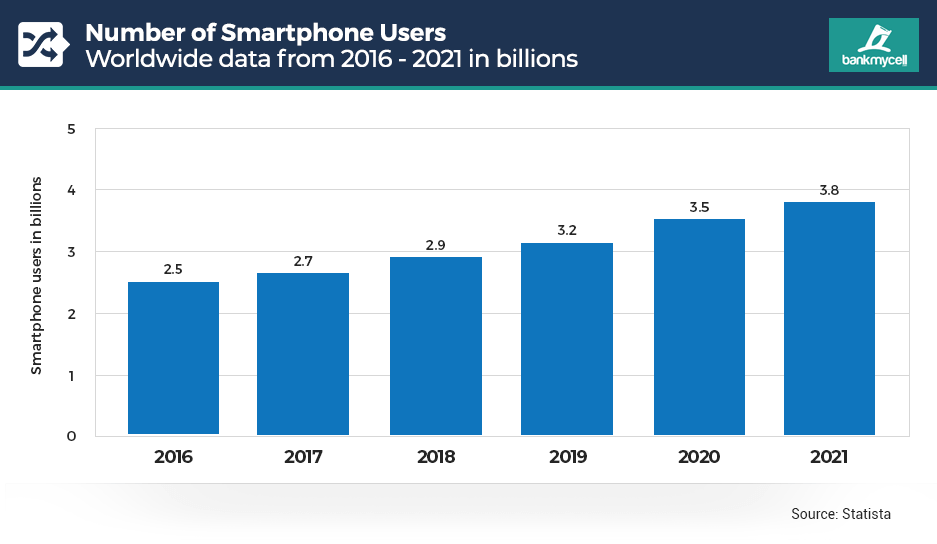
\includegraphics[width=\textwidth]{img/smartphone_users}
\caption{Numero di utilizzatori di smartphone nel mondo \cite{bankmycell}}
\label{fig:smartphone_users}
\end{figure}

\section{mHealth}
Lo sviluppo di questi studi e la diffusione degli smartphone nel mondo ha portato a quella che è chiamata \textbf{mHealth} \textit{(o mobile health)}; la messa in pratica della medicina e della salute pubblica supportata dall'utilizzo di dispositivi mobile\cite{mHealth}.
La mHealth è una parte di quella che viene chiamata \textbf{eHealth}, ovvero l'utilizzo di dispositivi informatici e tecnologici \textit{(dai computer ai monitor dei pazienti)} per il supporto dei servizi salutari.
Questo tipo di tecnologie permette oggi anche a paesi sottosviluppati di avere accesso ad una assistenza sanitaria di qualche tipo per permettere di identificare e curare in tempo eventuali disturbi.

Tra i vari servizi resi disponibili dalla mHealth ci sono anche quelli \textbf{educativi} del paziente sui disturbi di cui soffre, quelli di \textbf{helpline} che forniscono al paziente un contatto con esperti del settore e quelli di \textbf{remote disease surveillance} che permettono al paziente di diventare consapevole dei propri disturbi ed eventualmente sostenere un percorso di guarigione \textit{(che sia online o meno)}, che è esattamente quello a cui miriamo con la nostra applicazione.

\section{Strategie Principali}
Come abbiamo detto, il vantaggio principale delle pratiche come mHealth sono l'accesso in
maniera anonima e la libera scelta di un orario, fattori sicuramente positivi per il target d'udienza dell'applicazione, ovvero gli studenti universitari.
Per quanto riguarda l'identificazione e lo sviluppo di cura dei disturbi psichici, alcune strategie chiave sono il \textbf{monitoraggio dell'umore} del soggetto, la raccomandazione di \textbf{attività che scoraggino i pensieri negativi}, l'\textbf{educazione} del soggetto sui propri disturbi e l'\textbf{accesso alle reti di supporto} da parte di esso; tutte queste strategie fanno parte della \textbf{Terapia Cognitivo-Comportamentale}\cite{CBT} che è un metodo di cura adatto al trattamento individuale ed è finalizzata a trattare i pensieri negativi, le emozioni disfunzionali e i comportamenti disadattivi del paziente in modo da facilitare l'eliminazione dei disturbi psicologici.

\section{Funzionalità Offerte}
Dunque, scopo finale dello stage è stato quello di realizzare un'applicazione di mHealth che permetta agli utenti, nel nostro caso agli studenti universitari, di auto-educarsi sui disturbi di cui potrebbero soffrire tramite un'attività iniziale di \textbf{screening} atta ad identificare segnali d'allarme che possano suggerire la presenza di tali disturbi, e l'eventuale \textbf{educazione} e \textbf{mitigazione} di essi tramite \textbf{attività di monitoraggio dell'umore}, \textbf{lezioni didattiche} sui propri disturbi e su come combatterli, \textbf{esercizi attivi} per il recupero.
Questo sarà eseguito utilizzando dei questionari accompagnati da contenuti multimediali da
completare settimanalmente, uniti a una parte di domande giornaliere per il monitoraggio
dell'utente. I questionari sono creati sulla piattaforma \textbf{Qualtrics}, nata inizialmente per gestire dei questionari di tipo aziendale, che permette di definire diversi tipi di domande e di inserire vari media nelle domande stesse, offrendo l'accesso a tutto ciò tramite API.
Verrà inoltre tenuta traccia dei progressi dell'utente e, utilizzando un calendario, verranno segnalati nuovi esercizi ogni volta che questi sono disponibili. Per permettere un monitoraggio del soggetto sono inoltre disponibili delle domande giornaliere che verranno notificate all'utente ad un orario a sua scelta.

